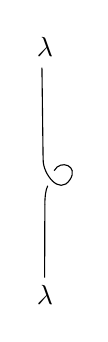
\begin{tikzpicture}[yscale=-1,scale=0.015,baseline={([yshift=-.5ex]current bounding box.center)}]
\begin{scope}[shift={(0.00mm,719.29mm)}]
% path id='path3342'
% path spec='M 684.88343,62.41273 C 683.01827,175.03224 820.64762,363.84276 911.1576,228.07775 988.63013,111.86895 831.68679,51.26311 777.81746,151.30615'
\draw [fill=none,draw=black] (684.88mm,62.41mm)
%%%% Warning: check controls
.. controls (683.02mm,175.03mm) and (820.65mm,363.84mm) .. (911.16mm,228.08mm)
%%%% Warning: check controls
.. controls (988.63mm,111.87mm) and (831.69mm,51.26mm) .. (777.82mm,151.31mm)
;
% path id='path3344'
% path spec='m 723.26922,278.58538 c -20.30486,42.58058 -24.24366,105.09648 -24.24366,157.58378'
\draw [fill=none,draw=black] (723.27mm,278.59mm)
.. controls ++(-20.30mm,42.58mm) and ++(0.00mm,-52.49mm) .. ++(-24.24mm,157.58mm)
;
% path id='path3346'
% path spec='m 684.28571,60.93365 -10,-781.42857'
\draw [fill=none,draw=black] (684.29mm,60.93mm)
-- ++(-10.00mm,-781.43mm)
;
% path id='path3348'
% path spec='m 699.02556,434.14886 -1.8827,622.49914'
\draw [fill=none,draw=black] (699.03mm,434.15mm)
-- ++(-1.88mm,622.50mm)
;
\node [black] at (700mm,-900mm) { $\lambda$ };
\node [black] at (700mm,1200mm) { $\lambda$ };
\end{scope}
\end{tikzpicture}
